
\chapter{Appendices for Multi-Regge theory} % Main appendix title
\label{AppendixMultiRegge}
%%%%%%%%%%%%%%%%%%%%%%%%%%%%%%%%
\section{Lightcone blocks}\label{app:Blocks}
%%%%%%%%%%%%%%%%%%%%%%%%%%%%%%%%
The scalar five-point conformal blocks, mentioned in the main text, can be expressed in terms of an expansion around the lightcone (\ref{eq:scalarblockslightcone})  by acting with (\ref{eq:lightconeScalarAll}) on a three-point function. In (\ref{eq:scalarblockslightcone})  we have written it in terms of a function $\tilde{\mathcal{I}}_{n_1,n_2}$ given by
\begin{align}
   & \tilde{\mathcal{I}}_{n_1,n_2}=\tfrac{\left(\frac{a-\Delta_5}{2}\right)_{n_1}\left(\frac{2 n_1-\Delta_5+a}{2} \right)_{n_2} \left(\frac{a+4-\Delta_5-d}{2} \right)_{n_1} \left(\frac{2 n_1-\Delta_5+a+4-d}{2} \right)_{n_2} }{  \left(t_1^2 u_1 u_4-t_1 \left(t_2 \left(1-u_5\right)+t_2 u_4 \left(u_2 u_5-1\right)+u_1 u_4+u_5-1\right)+u_5 \left(t_2^2 u_3-t_2 \left(u_3-u_2 u_4+1\right)+1\right)\right)^{\frac{a+2 n_1+2 n_2-\Delta_5}{2}} } \label{eq:blockscalarposallmi} \\
   & \prod_{i=1}^2\tfrac{(-1)^{n_i} \Gamma (2 n_i+\Delta_{k_i})  \left(\frac{\Delta_{k_i}}{2}\right)_{n_i}^2  (t_i(1-t_i))^{\frac{\Delta_{k_i}+2n_i}{2}-1}    }{n_i!(\Delta_{k_i})_{2 n_i} \left(\frac{2\Delta_{k_i}+4-d }{2}\right)_{n_i} \Gamma^2 \left(\frac{2n_i+\Delta_{k_i}}{2}\right) }\nonumber
\end{align}
%{\bf Verify}
where $a=\Delta_{k_1}+\Delta_{k_2}$. One nice feature of this result is that it allows to to analytic continuations in $u_2,u_4,u_5$ at all orders in $u_1$ and $u_3$, this is specially useful to verify that the analytic continuation of the conformal block has a distinct behavior in the Regge limit. With this expression in our hands we can also do a Mellin transform and obtain the Mellin amplitude associated with the scalar conformal block. For  instance the function $Q_{m_1,m_2}$ in (\ref{eq:MellinamplitudepolesQ}) is given in this case by
\begin{align}
   & Q_{m_1,m_2}=\sum_{n_i=0}\prod_{i=1}^2\tfrac{2(-1)^{m_i} \Gamma \left(\Delta _{k_i}\right) }{ \left(m_i-n_i\right)! \Gamma^2 \left(\frac{\Delta _{k_i}}{2}\right) \Gamma \left(\Delta_{\phi}-m_i-\frac{\Delta _{k_i}}{2}\right)  \left(1-\frac{d }{2}+\Delta _{k_i}\right)_{m_i-n_i}  }\tfrac{\left(\frac{\bar{\Delta} -\Delta_{\phi} }{2} \right)_{m_1-n_1} \binom{n_1+n_2+\frac{\Delta_{\phi}}{2}-m_1-m_2-\frac{\bar{\Delta} }{2}  }{n_1}}{   \Gamma \left(\frac{\Delta_{\phi}+2 m_1-2 m_2+\Delta _{k_1}-\Delta _{k_2}}{2} \right)  }\nonumber \\
   & \times\tfrac{ \left(\frac{\bar{\Delta}+2-d -\Delta_{\phi}}{2} \right)_{m_1-n_1} \left(\frac{2 m_1+\bar{\Delta}-2 n_1-\Delta_{\phi}}{2}  \right)_{m_2-n_2} \left(\frac{2 m_1+\bar{\Delta}+2 -d -2 n_1-\Delta_{\phi}}{2}  \right)_{m_2-n_2} \binom{\frac{2 n_2+\Delta_{\phi}-2 m_1-2 m_2-\bar{\Delta} }{2} }{n_2}  }{   \Gamma \left(\frac{\Delta_{\phi}-2 m_1+2 m_2-\Delta _{k_1}+\Delta _{k_2} }{2} \right) \Gamma \left(\frac{2 m_1+2 m_2+\bar{\Delta} -\Delta_{\phi}}{2} \right) }\label{eq:ScalarblockMellin}
\end{align}
where $\bar{\Delta}=\Delta_{k_1}+\Delta_{k_2}$. Note that it does not depend on the variables $s_{ij}$ as expected since the exchanged operators are scalars. The apparent asymetry in the channels $(12)$ and $(34)$ is related with the choice of which differential operator $F_k$ we decide to act first on a three-point function. Another advantage of having the Mellin amplitude for the scalar conformal block is that it can be used to generate some solutions for spinning blocks as we have shown in section \ref{sec:MellinMellin}.

We have checked that the solution (\ref{eq:ScalarblockMellin}) satisfies the Casimir recurrence equation, in the channel $(12)$,    given by 
%{\bf JVB: Isn't there an f missing after each $\mathbf{d}$ in the expression. Other possibility is to use the same notation as in main text.}
\begin{align}
   & \big[\mathbf{d}_{00000} \big(2 \textrm{c}_{\Delta_1J_1}-a_1^2+a_1 (2 a_4+a_5-a_3-2 d+3 \Delta_\phi )-2 a_2 (a_3+a_4)+2 a_3^2-2 a_3 a_4-2 a_3 a_5\nonumber                 \\
   & +\Delta_\phi  (5 a_3-4 a_4-2 a_5+4 d)+2 a_4^2+a_4 a_5-2 \Delta_\phi ^2\big)\nonumber\\
   &+\mathbf{d}_{00-200} (a_1-a_3+a_4-2 \Delta_\phi ) (a_3-2 a_2-a_5+2 \Delta_\phi )\nonumber \\
   & -\mathbf{d}_{000-20} (a_1-2 a_2+a_4-\Delta_\phi ) (a_1-a_3+a_4-2 \Delta_\phi )-a_3 \mathbf{d}_{002-20} (a_1-2 a_2+a_4-\Delta_\phi )\nonumber                         \\
   & +a_1 \mathbf{d}_{-2000-2} (a_1-2 a_2-a_5+\Delta_\phi )+a_1 \mathbf{d}_{-2002-2} (a_1-2 a_2-a_5+\Delta_\phi )+2 a_1 a_2 \mathbf{d}_{-2-2-200}\nonumber                \\
   & +2 a_1 a_2 \mathbf{d}_{-2-2000}+a_1 a_5 \mathbf{d}_{-20-220}+a_1 a_5 \mathbf{d}_{-20000}+a_4 \mathbf{d}_{00-220} (2 a_2-a_3+a_5-2 \Delta_\phi )\nonumber             \\
   & +a_4 \mathbf{d}_{00020} (a_3-a_4-a_5+\Delta_\phi )+a_3 \mathbf{d}_{00200} (a_4+a_5-a_3-\Delta_\phi )\big]f(t_{ij},s_{ij})=0\label{eq:recurrencerelationsMellinCasi}
\end{align}
where $\mathbf{d}_{i_1i_2i_3i_4i_5}$ is defined by $\mathbf{d}_{i_1i_2i_3i_4i_5}f(t_{12},t_{34},s_{13},s_{25},s_{45})=f(t_{12}+i_1,\dots,s_{45}+i_5)$ and the coefficients $a_i$ are given by
\begin{align}
   & a_1= 2 \Delta_\phi -t_{12},\, \ \ \  a_2= \frac{2 \Delta_\phi -t_{34}}{2} ,\, \ \ \ a_3 =  \Delta_\phi -s_{13}, \\
   & a_4= s_{25}+t_{12}-t_{34}+\Delta_\phi ,\, \ \ a_5=  s_{45}-t_{12}+t_{34}+\Delta_\phi\,.\nonumber
\end{align}
This recurrence relation is also valid for spinning conformal blocks.
%%%%%%%%%%%%%%%%%%%%%%%%%%%%%%%%%
\subsection{Spinning recursion relations}
%%%%%%%%%%%%%%%%%%%%%%%%%%%%%%%%%
In \cite{Poland:2021xjs} the authors have derived identities that blocks with different values of spin satisfy. It is possible to verify part of these relations using lightcone blocks for unequal external dimensions introduced in the previous subsection. Using (\ref{eq:lightconeLeadingSpin}) we can verify that the lightcone blocks satisfy
\begin{align}
   & (2 J_1+2 \ell+\tau_1+\tau_2-2-\Delta_5) G_{\tau_1,J_1,\tau_2,J_2,\ell}^{\Delta_{1},\Delta_5,\Delta_3}
  % -\frac{4 (2 J_1+\tau_1-2) (2 J_1+\tau_1-1) G_{\tau_1,J_1-1,\tau_2,J_2,\ell}^{\Delta_{1},\Delta_5,\Delta_3}}{(2 J_1+\tau_1-\Delta_{12}-2) (2 J_1+2 \ell+\tau_1+\tau_2-\Delta_5-2)}
  + 2 (J_2-\ell) G_{\tau_1,J_1,\tau_2,J_2,\ell+1}^{\Delta_{1},\Delta_5,\Delta_3}
  %+\frac{2 (J_2-l) G_{\tau_1,J_1,\tau_2,J_2,\ell+1}^{\Delta_{1},\Delta_5,\Delta_3} }{2 J_1+2 \ell+\tau_1+\tau_2-\Delta_5-2}
  \label{eq:RecurrencerelationJ}                                                                                                                                                                                                                                              \\
   & +\frac{4 (2 J_1+\tau_1-2) (2 J_1+\tau_1-1) }{(2 J_1+\tau_1-\Delta_{12}-2) }\bigg[\frac{\sqrt{u_5}  G_{\tau_1+1,J_1-1,\tau_2,J_2,\ell}^{\Delta_{1}+1,\Delta_5+1,\Delta_3} }{\sqrt{u_1} }-G_{\tau_1,J_1-1,\tau_2,J_2,\ell}^{\Delta_{1},\Delta_5,\Delta_3}\bigg]=0\nonumber
\end{align}
where $G_{\tau_1,J_1,\tau_2,J_2,\ell}^{\Delta_1,\Delta_5,\Delta_3}$ represents the lightcone conformal block for the exchange of a twist $\tau_i$ and spin $J_i$ in the channels $(12)$ and $(34)$ for external with dimension $\Delta_i$,\begin{align}
   & G_{\tau_1,J_1,\tau_2,J_2,\ell}^{\Delta_1,\Delta_5,\Delta_3} =  u_1^{\frac{\tau_1}{2}}  u_3^{\frac{\tau_2}{2}}u_5^{\frac{\Delta_5}{2}}(1-u_2)^{\ell} \int [dt_1dt_2] (1-u_2 u_5+t_2 (u_2-1) u_5)^{J_1-\ell }                                                                  \\
   & \tfrac{(1-u_2 u_4+t_1 (u_2-1) u_4)^{J_2-\ell } }{(1+t_1 (u_5-1))^{\frac{\Delta_5+2 J_1+\tau_1-\tau_2-2 \ell }{2} }  (1+t_2 (u_4-1))^{\frac{\Delta_5+2 J_2-\tau_1+\tau_2-2 \ell}{2}}  (1+(1-t_1) (1-t_2) (u_2-1))^{\frac{2 J_1+2 J_2+\tau_1+\tau_2-\Delta_5}{2} } } \nonumber
\end{align}
where $[dt_1dt_2] = \prod_{i=1}^2\frac{dt_i\,\Gamma(2J_i+\tau_i)t^{\frac{\tau_i+2J_i+a_i}{2}-1}(1-t_i)^{\frac{\tau_i+2J_i-a_i}{2}-1}}{\Gamma\left(\frac{\tau_i+2J_i+a_i}{2}\right)\Gamma\left(\frac{\tau_i+2J_i-a_i}{2}\right) }$ with $a_1=\Delta_{12}, a_2=\Delta_{34}$.
As before, the index $\ell$ labels a particular structure in the three-point function (\ref{eq:threepontfunction}) 
%{\bf JVB: Do you need it here. Above you want to reference this equation or the one in the main text? Here I suppose you want to reference (\ref{eq:threepontfunction})}

 By considering the Mellin transform of $G_{\tau_1,J_1,\tau_2,J_2,\ell}^{\Delta_1,\Delta_5,\Delta_3}$ we can phrase the recurrence relation in spin (\ref{eq:RecurrencerelationJ})  in terms of a Mellin amplitudes
\begin{align}
   & \frac{2 (2 J_1+\tau_1-2) (2 J_1+\tau_1-1) ((\Delta_5-2 \delta_{25}+\tau_{12}) \mathcal{M}_{\tau_1+1,J_1-1,\tau_2,J_2,l}^{\Delta_1+1,\Delta_5+1,\Delta_3}-\mathcal{M}_{\tau_1,J_1-1,\tau_2,J_2,\ell}^{\Delta_1,\Delta_5,\Delta_3})}{(2 J_1+\tau_1-\Delta_{12}-2) } \nonumber \\
  %& +\frac{2 (2 J_1+\tau_1-2) (2 J_1+\tau_1-1) (\Delta_5-2 \delta_{25}+\tau_{12}) \mathcal{M}_{\tau_1+1,J_1-1,\tau_2,J_2,l}^{\Delta_1+1,\Delta_5+1,\Delta_3}  }{(2 J_1+\tau_1-\Delta_{12}-2) (2 J_1+2 l+\tau_1+\tau_2-\Delta_5-2)}
   & +(2 J_1+2 \ell+\tau_1+\tau_2-\Delta_5-2)\mathcal{M}_{\tau_1,J_1,\tau_2,J_2,\ell}^{\Delta_1,\Delta_5,\Delta_3}+2 (J_2-\ell) \mathcal{M}_{\tau_1,J_1,\tau_2,J_2,\ell+1}^{\Delta_1,\Delta_5,\Delta_3}=0\label{eq:MellinRecurrencespin}
\end{align}
with
\begin{align}
  G_{\tau_1,J_1,\tau_2,J_2,\ell}^{\Delta_1,\Delta_5,\Delta_3} = u_1^{\frac{\tau_1}{2}}  u_3^{\frac{\tau_2}{2}}\! \int [d\delta_{ij}] \mathcal{M}_{\tau_1,J_1,\tau_2,J_2,\ell}^{\Delta_1,\Delta_5,\Delta_3}(\delta_{ij})  u_4^{-\delta_{45}} u_5^{\delta_{ 25}+\frac{ \tau_2-\tau_1 }{2}} u_2^{\delta_{13} -\delta_{45} +\frac{\Delta_5-a_2-\tau_1}{2}} \prod_{i<j}\Gamma(\delta_{ij})
\end{align}
where we have used the constraints to eliminate the some of the $\delta_{ij}$ and $\delta_{12}$ and $\delta_{34}$ are set to $\frac{\Delta_1+\Delta_2-\tau_1}{2}$ and $\frac{\Delta_3+\Delta_4-\tau_2}{2}$ respectively. We have suppressed the dependence on Mellin variables in (\ref{eq:MellinRecurrencespin}) since there are no shifts in them.


There is an extra identity that is needed to turn (\ref{eq:RecurrencerelationJ}) into a self-consistent recurrence relation
\begin{align}
   & \frac{4 (\tau_1+2 \ell -1) (\tau_2+2 \ell -1) (\tau_1+\tau_2+4 \ell-\Delta_5 -4) }{(\tau_1+2 \ell-\Delta_{12} -2) (\Delta_{34}+\tau_2+2 \ell -2) }\bigg[\frac{G_{\tau_1+1,\ell -1,\tau_2+1,\ell -1,\ell -1}^{\Delta_1+1,\Delta_5,\Delta_3-1}}{\sqrt{u_1} \sqrt{u_3} }-G_{\tau_1,\ell -1,\tau_2,\ell -1,\ell -1}^{\Delta_1,\Delta_5,\Delta_3}\bigg]\nonumber   \\
   & +\frac{ (\Delta_5-\tau_{12}) (\tau_1+2 \ell -1)  }{(\tau_2+2 \ell -2) (\tau_1+2 \ell-\Delta_{12} -2)}    \bigg[\frac{\sqrt{u_5} (\Delta_5+\tau_{12}) G_{\tau_1+1,\ell -1,\tau_2,\ell ,\ell -1}^{\Delta_1+1,\Delta_5+1,\Delta_3}}{\sqrt{u_1} }-2G_{\tau_1,\ell -1,\tau_2,\ell ,\ell -1}^{\Delta_1,\Delta_5,\Delta_3}\bigg]                           \nonumber \\
  %	 & -\frac{4 (\tau_1+2 \ell -1) (\tau_2+2 \ell -1) (\tau_1+\tau_2+4 \ell-\Delta_5 -4) G_{\tau_1,\ell -1,\tau_2,\ell -1,\ell -1}^{\Delta_1,\Delta_5,\Delta_3} }{(\tau_1+2 \ell-\Delta_{12} -2) (\Delta_{34}+\tau_2+2 \ell -2) (\tau_1+\tau_2+4 \ell-\Delta_5 -2)}\nonumber                           \\
  %	 & -\frac{2 (\Delta_5-\tau_{12}) (\tau_1+2 \ell -2) (\tau_1+2 \ell -1)  }{(\tau_2+2 \ell -2) (\tau_1+2 \ell-\Delta_{12} -2) (\tau_1+\tau_2+4 \ell-\Delta_5 -2)}\nonumber                                                        \\
   & -\frac{(\Delta_5+\tau_{12}) (\tau_2+2 \ell -1) (\tau_1+\tau_2+4 \ell-\Delta_5 -4) G_{\tau_1,\ell ,\tau_2,\ell -1,\ell -1}^{\Delta_1,\Delta_5,\Delta_3}}{(\tau_1+2 \ell -2) (\Delta_{34}+\tau_2+2 \ell -2)}\nonumber                                                                                                                                          \\
   & + (\tau_1+\tau_2+4 \ell -\Delta_5-2)G_{\tau_1,\ell ,\tau_2,\ell,\ell }^{\Delta_1,\Delta_5,\Delta_3} =0.
\end{align}

%It is possible to find some solutions for simple cases of this difference equation. Take $m_1=m_2$ then the solution that does not involve $s_{13}$ is given by
%\begin{align}
%	Q_{0,0}(s_{25},s_{45}) = & \,_3F_2\left(-J_1,J_1+\tau_1-1,\Delta_{\phi}-\frac{s_{25}}{2};\frac{\tau_1}{2},\frac{\Delta_{\phi}-\tau_{21}}{2};1\right)\times     \\
%	                         & \,_3F_2\left(-J_2,J_2+\tau_2-1,\Delta_{\phi}-\frac{s_{45}}{2};\frac{\tau_2}{2},\frac{\Delta_{\phi}-\tau_{12}}{2};1\right).\nonumber
%\end{align}
%This result is quite similar to the four point Mack polynomial, see for instance eq. (127) \cite{Costa:2012cb}. This confirms the expectation that $s_{13} =0$ leads to a product two four point independent kinematics.



%%%%%%%%%%%%%%%%%%%%
%\subsection{Conformal partial wave}
%%%%%%%%%%%%%%%%%%%%%
%First one starts by acting with $D_{z}$ and removing the null polarizations vectors $z$. As explained in \ref{subsec:Euclideanlimitsubsection} this gives rise to a polynomial  $\mathcal{H}^{\ell}$ in three variables $\xi_i$
%\begin{align}
%&F_{\nu_1,\nu_2,J_1,J_2}^{\ell} =\int {{\scriptscriptstyle \frac{d^dx_6 d^dx_{7}\,\,\, (x_{12}^2)^{\frac{\tau_1}{2}}(x_{34}^2)^{\frac{\tau_2}{2}} \mathcal{H}_{J_1,J_2}^{\ell}(\xi_1,\xi_2,\xi_3)}{(x_{16}^2)^{\frac{h+i\nu_1}{2}}(x_{26}^2)^{\frac{h+i\nu_1}{2}}(x_{37}^2)^{\frac{h+i\nu_2}{2}}(x_{47}^2)^{\frac{h+i\nu_2}{2}}(x_{67}^2)^{\frac{2h-i(\nu_1+\nu_2)-\Delta_\phi}{2}}(x_{56}^2)^{\frac{i\nu_{21}+\Delta_\phi}{2}}(x_{57}^2)^{\frac{i\nu_{12}+\Delta_\phi}{2}} } }}\nonumber
%\end{align}
%where $h\equiv \frac{d}{2},\tau_i=\equiv = h+i\nu_i-J_i$ and the variables $\xi_i$ are given by
%\begin{align}
%&\xi_1= {{\scriptscriptstyle\frac{x_{26}^2(x_{67}^2x_{15}^2-x_{56}^2x_{17}^2)+x_{16}^2(x_{56}^2x_{27}^2-x_{25}^2x_{67}^2)}{(x_{16}^2x_{26}^2x_{12}^2x_{56}^2x_{67}^2x_{57}^2)^{\frac{1}{2}}}}},\,\xi_2=  {{\scriptscriptstyle\frac{x_{47}^2(x_{67}^2x_{35}^2-x_{57}^2x_{36}^2)+x_{37}^2(x_{57}^2x_{46}^2-x_{45}^2x_{67}^2)}{(x_{37}^2x_{47}^2x_{34}^2x_{57}^2x_{67}^2x_{56}^2)^{\frac{1}{2}}}}}\nonumber\\
%&\xi_3={{\scriptscriptstyle \frac{x_{26}^2(x_{17}^2(x_{46}^2x_{37}^2-x_{36}^2x_{47}^2)+x_{67}^2(x_{13}^2x_{47}^2-x_{14}^2x_{37}^2))+x_{16}^2(x_{27}^2(x_{36}^2x_{47}^2-x_{46}^2x_{37}^2)+x_{67}^2(x_{24}^2x_{37}^2-x_{23}^2x_{47}^2))}{(x_{16}^2x_{26}^2x_{67}^4x_{12}^2x_{34}^2x_{37}^2x_{47}^2)^{\frac{1}{2}}}}}\nonumber.
%\end{align}
%The different solutions in (\ref{eq:conformalpartialwave}) have distinct behaviours in the $u_1,u_3\rightarrow 0$ limit. So by analyzing the integral representation in this limit it is possible to read off the coefficients $c_i$ appearing (\ref{eq:conformalpartialwave}).  In this limit the angular part simplifies to $\mathcal{H}^{\ell}_{J_i} \rightarrow \xi_1^{J_1-\ell}\xi_2^{J_2-\ell}\xi_3^{\ell}$
%\begin{align}
%&F_{\nu_1,\nu_2,J_1,J_2}^{\ell} \rightarrow \int {{ \frac{d^dx_6 d^dx_{7}\,\,\, (x_{12}^2)^{\frac{\tau_1}{2}}(x_{34}^2)^{\frac{\tau_2}{2}} \xi_1^{J_1-\ell}\xi_2^{J_2-\ell}\xi_3^{\ell} }{(x_{16}^2)^{\frac{h+i\nu_1}{2}}(x_{26}^2)^{\frac{h+i\nu_1}{2}}(x_{37}^2)^{\frac{h+i\nu_2}{2}}(x_{47}^2)^{\frac{h+i\nu_2}{2}}(x_{67}^2)^{\frac{2h-i(\nu_1+\nu_2)-\Delta_\phi}{2}} (x_{56}^2)^{\frac{i\nu_{21}+\Delta_\phi}{2}}(x_{57}^2)^{\frac{i\nu_{12}+\Delta_\phi}{2}}  }  }}\nonumber
%\end{align}
%Now we can introduce Feynman parameters and  

\section{Scalar Mellin partial-wave}\label{app:ScaMellinpar}
In this appendix, we derive the Mellin partial-wave for scalar exchange within a five-point function. We start from partial-wave definition in position space
\begin{equation}
 	F_{\nu_1, \nu_2,0,0,0}(x_i)=\int dx_6 dx_7 \langle\phi_{1}\phi_2 \phi(x_6)\rangle\langle\tilde{\phi}(x_6)\phi_5 \tilde{\phi}(x_7)\rangle\langle\phi_{3}\phi_4 \phi(x_7)\rangle
\end{equation}
where the subscripts ans superscript $0$ in $F_{\nu_1, \nu_2,0,0,0}$ denote the scalar exchanges and the superscripts refer to principal series representations of the exchanged operators. The notation $\langle \phi_i \phi_j \phi_k\rangle$ denotes kinematical structure of three-point functions
\begin{align}
  \langle\phi_1 \phi_2 \phi_3\rangle=\frac{1}{\left(-2P_{1}\cdot P_{2}\right)^{\frac{1}{2}(\Delta_1+\Delta_2-\Delta_3)}\left(-2P_{1}\cdot P_{3}\right)^{\frac{1}{2}(\Delta_1+\Delta_3-\Delta_2)}\left(-2P_{2}\cdot P_{3}\right)^{\frac{1}{2}(\Delta_2+\Delta_2-\Delta_1)}}\,,
\end{align}
where we use embedding space where $-2 P_{i}\cdot P_{j}=x_{ij}^2$.
Note that as we only consider scalar exchanges there is no sum over different possible tensor structures. In general, we consider unequal scalar fields labelled by their scaling dimensions $\Delta_i$. For operators of fixed position we do the abuse of notation $\phi_i\equiv\phi(x_i)$ but we retain the dependence on integrated variables using $\phi(x_i)$. The latter notation corresponds to scalar operators of scaling dimension $h+i \nu_i$ with $h=d/2$. Moreover, shadow operators of scaling dimension $h-i \nu_i$ are denoted with an extra tilde.

In order to integrate over $x_6$ and $x_7$ we use the Schwinger parametrization
\begin{align}
  \label{eq:schwingerparam}
  \frac{1}{(-2 P_{i}\cdot P_j)^a}=\frac{1}{\Gamma\left(m+a\right)}\int_{0}^{\infty} \frac{dt_{ij}}{t_{ij}}\, t_{ij}^{m+a}(-\partial_{t_{ij}})^{m} e^{2t_{ij} P_{i}\cdot P_j}\,.
\end{align}
for any power $a$, $(-P_{i}\cdot P_j)>0$ and some integer $m$ such that $\text{Re}(m+a)>0$. For our purposes here, it is enough to take $m=0$. It will also be useful to consider the following change of variables
\begin{align}
  \label{eq:changevariablests}
   & t_{12}=2 t_1 t_2\,,\quad t_{16}=2 t_1 t \,,\quad t_{26}=2 t_2 t \,, \quad t_{34}= 2 t_3 t_4\,,\quad t_{37}=2 t_3 s\,,\nonumber \\
   & t_{47}=2 t_4 s\,,\quad t_{56}=2 t_5 \bar{t}\,,\quad t_{57}=2 t_5 \bar{s}\,,\quad t_{67}=2 \bar{t} \bar{s}\,,
\end{align}
which is introduced to reproduce the form of integral one finds from considering a tree-level Witten diagram with two scalar exchanges using the notation of~\cite{Penedones:2010ue}. Here $t_i$'s are related with bulk-to-boundary propagators of the external scalars whereas $t, \bar{t}, s, \bar{s}$ refer to split representations of the bulk-to-bulk propagators.

The integrals over $x_6$ and $x_7$ are easy to compute successively by noting~\cite{Penedones:2010ue}
\begin{equation}
  \int_{0}^{\infty} \frac{dt d\bar{t}}{t \bar{t}} t^{\Delta_t} \bar{t}^{\Delta_{\bar{t}}} \int dP e^{2 P\cdot (t X+ \bar{t} Y)} = 2 \pi^{h}\int_{0}^{\infty} \frac{dt d\bar{t}}{t \bar{t}} t^{\Delta_t}\bar{t}^{\Delta_{\bar{t}}} e^{(t X+ \bar{t} Y)^2}
\end{equation}
where $\Delta_{t}+\Delta_{\bar{t}}= 2h$ with $X$ and $Y$ two timelike vectors.
We then find (dropping constants)
\begin{align}
   & F_{\nu_1, \nu_2,0,0}^{0}(x_i)\sim \int \frac{dt d\bar{t} ds d\bar{s}}{t\bar{t} s \bar{s}}t^{h+i \nu_1} \bar{t}^{h-i\nu_1} s^{h+i\nu_2} \bar{s}^{h-i\nu_2}
 \nonumber\\  
   &\left(\prod_{i=1}^{5}\int\frac{dt_i}{t_i} t_i^{\Delta_i}\right) \exp\left[-t_1 t_2 x_{12}^2 \left(t^2 \left(\bar{s}^2 \bar{t}^2+1\right)+1\right)\right.\nonumber \\
   & \left.-t_1 t_3 x_{13}^2 t\bar{t} s \bar{s}-t_1 t_4 x_{14}^2 t \bar{t} s \bar{s}- t_1 t_5 x_{15}^2 t \bar{t}
  \left(\bar{s}^2 \left(\bar{t}^2+1\right)+1\right)- t_2 t_3 x_{23}^2 t \bar{t} s \bar{s}-t_2 t_4 x_{24}^2 t  \bar{t} s \bar{s}\right.\nonumber                                                                                                                                                                               \\
   & \left.-t_2 t_5 x_{25}^2 t \bar{t} \left(\bar{s}^2
    \left(\bar{t}^2+1\right)+1\right)-t_3 t_4 x_{34}^2 \left(s^2+1\right)- t_3 t_5 x_{35}^2 s
    \bar{s} \left(\bar{t}^2+1\right)- t_4 t_5  x_{45}^2 s \bar{s} \left(\bar{t}^2+1\right)\right]
\end{align}
which is of the form of Symanzik's formula~\cite{Symanzik:1972wj}
\begin{equation}
  \label{eq:symanzikformula}
  2\int_{0}^{\infty}\prod_{i=1}^{n}\frac{dt_i}{t_i}t_i^{\Delta_i}e^{-\sum_{i<j}^{n} t_i t_j Q_{ij}}=\frac{1}{(2\pi i)^{(n(n-3))/2}}\int d\delta_{ij}\prod_{i<j}^{n}\Gamma(\delta_{ij})Q_{ij}^{-\delta_{ij}}\,,
\end{equation}
with $Q_{ij}>0$. The Mellin variables $\delta_{ij}$ are integrated along a contour parallel to the imaginary axis with $\text{Re} (\delta_{ij})>0$ and obey the constraints
\begin{equation}
  \sum_{j\ne i}^{n}\delta_{ij}=\Delta_i\,.
\end{equation}
This allows us to find the inverse Mellin transform of the position-space partial-wave and the Mellin partial-wave
\begin{align}
  F_{\nu_1, \nu_2,0,0,0}(x_i)= \frac{1}{(2\pi i)^5}\int d\delta_{ij}  \mathcal{M}_{\nu_1, \nu_2,0,0,0}(\delta_{ij})\prod_{i<j}^{n}\Gamma(\delta_{ij})x_{ij}^{-2\delta_{ij}}
\end{align}
The remaining integrations in $t, \bar{t}, s$ and $\bar{s}$ are straightforward to do. We then find
\begin{align}
  \mathcal{M}_{\nu_1, \nu_2,0,0,0}(\delta_{ij})= & {\textstyle\frac{\pi^{2h}\left(\left(\prod_{i=1}^{2}\Gamma\left(\frac{\Delta_{2i-1}+\Delta_{2i}-t_{2i-1\,2i}}{2}\right)\left(\prod_{\sigma=\pm}\Gamma\left(\frac{h+\sigma \left(\Delta_{2i-1}-\Delta_{2i}\right)+i \nu_i}{2}\right)\right)\right)\right)^{-1}}{\Gamma \left(\Delta _5\right) \Gamma \left(\frac{\Delta _5-i \nu _1+i \nu _2}{2}\right) \Gamma \left(\frac{t_{12}-t_{34}+\Delta _5}{2}\right) \Gamma \left(\frac{2 h-\Delta _5-i \nu _1-i \nu _2}{2}\right) \Gamma \left(\frac{h-t_{12}+\Delta _5-i \nu _2}{2}\right)}} \\
                                       & {\textstyle\left[\left(\prod_{\sigma=\pm}\Gamma\left(\frac{h-t_{12}+\sigma\Delta_5-i \nu_2}{2}\right)\Gamma\left(\frac{\Delta_5+\sigma i \nu_1+i \nu_2}{2}\right)\right)\Gamma\left(\frac{h-t_{34}+i \nu_2}{2}\right)\Gamma\left(\frac{t_{12}-t_{34}+\Delta_5}{2}\right)\right.}\nonumber                                                                                                                                                                                                                                                       \\
                                       & {\textstyle\left. _3F_2\left(_{\Delta_5\,,\frac{2-h+t_{12}+\Delta_5+i\nu_2}{2}}^{\frac{t_{12}-t_{34}+\Delta_5}{2}\,,\frac{\Delta_5-i \nu_1+i \nu_2}{2},\frac{\Delta_5+i \nu_1+i \nu_2}{2}};1\right)+\Gamma\left(\Delta_5\right)\Gamma\left(\frac{t_{12}-h+\Delta_5+i \nu_2}{2}\right)\right.}\nonumber                                                                                                                                                                                                                                          \\
                                       & {\textstyle \left.\left(\prod_{\sigma=\pm}\prod_{i=1}^{2}\Gamma\left(\frac{h-t_{2i-1\,2i}+\sigma i\nu_i}{2}\right)\right)\,_3F_2\left(_{\frac{2+h-t_{12}-\Delta_5-i\nu_2}{2}\,,\frac{h-t_{12}+\Delta_5-i\nu_2}{2}}^{\frac{h-t_{12}-i\nu_1}{2}\,,\frac{h-t_{12}+i\nu_1}{2}\,,\frac{h-t_{34}-i\nu_2}{2}};1\right)\right]}\nonumber
\end{align}
where we use the notation $\delta_{ij}=\frac{\Delta_i+\Delta_j-t_{ij}}{2}$.

Let us finish this appendix by noting that a similar computation can be performed for spinning exchanges using Schwinger parametrization~(\ref{eq:schwingerparam}). To do so, at each moment, we multinomially expand the integrand decomposing it into sums over integrands of similar form to the ones encountered for scalar exchanges. In the end, one finds a spinning Mellin partial wave written as several sums over scalar-type Mellin partial waves. In particular the sums are bounded by the values of spin of the exchanged operators. This is no-good for an analytic continuation in spin that we want to consider here. For that reason and due to its length we do not write that result here.

\section{Explicit examples in position space}
In this appendix, we single-out a conformal block contribution in position space and compute its Regge-limit behaviour.

We start with five-point conformal block lightcone limit in its integral representation
\begin{align}
   & G_{k_1k_2\ell}(u_i)= u_1^\frac{\tau_1}{2} u_3^\frac{\tau_2}{2} (1-u_2)^{\ell} u_5^{\frac{\Delta_\phi}{2}} \int_{0}^{1} [dt_1][dt_2]
  \label{eq:5ptlightconeblockdef}                                                                                                                                                                                                                                                                       \\
   & \frac{\big(1-t_1(1-u_2)u_4-u_2u_4\big)^{J_2-\ell}\big(1-t_2(1-u_2)u_5-u_2u_5\big)^{J_1-\ell}}{\big(1-(1-u_4)t_2\big)^{\frac{h_2-\tau_1-2\ell+\Delta_\phi}{2}}\big(1-(1-u_5)t_1\big)^{\frac{h_1-\tau_2-2\ell+\Delta_\phi}{2}} \big(1-(1-t_1)(1-t_2)(1-u_2)\big)^{\frac{h_1+h_2-\Delta_\phi}{2}}}\,,
  \nonumber
\end{align}
where $\tau_i=\Delta_i-J_i$ is the twist and $h_i=\Delta_i+J_i$ the conformal spin of the $i$-th exchanged operator.
The measure is given by $[dt]=\frac{\Gamma(\Delta_i+J_i)}{\Gamma^2(\frac{\Delta_i+J_i}{2})}(t(1-t))^{\frac{\Delta_i+J_i}{2}-1}$.

Generically, we do not know how to evaluate these integrals in terms of known analytic functions.
However, when the exponents in the denominator of the integrand are integers, this is no longer the case.\footnote{The package HyperInt~\cite{Panzer:2014caa} is particularly useful to evaluate these integrals.} As a matter of example we consider the simple case of $\Delta_i=\Delta_\phi=2$ and $J_1=J_2=\ell=0$. Note that this is just a choice and spinning cases would also have a similar discussion but with longer explicit expressions. In this case, equation~\eqref{eq:5ptlightconeblockdef} can be integrated and yields (apart from an overall constant)
\begin{align}
  \label{eq:simplecase}
   & \frac{u_1 u_3 u_5}{1-u_5+u_4 \left(u_2 u_5-1\right)}
  \left[\text{Li}_2\left(u_2 u_4\right)-\text{Li}_2\left(u_4\right)+\text{Li}_2\left(u_2 u_5\right)-\text{Li}_2\left(u_5\right)-\text{Li}_2\left(u_2\right)\right.    \\
   & \left.-\log \left(1-u_2\right) \log \left(u_2\right)-\log \left(1-u_4\right) \log \left(u_4\right)-\log \left(1-u_5\right) \log \left(u_5\right)\right.\nonumber \\
   & \left.+\log \left(u_4\right)
    \log \left(u_5\right)+\log
    \left(u_2 u_5\right) \log \left(1-u_2 u_5\right)+\log
    \left(u_2 u_4\right)\log \left(1-u_2 u_4\right)+\zeta(2)\right]\nonumber\,.
\end{align}

As we perform the analytic continuation from an Euclidean to double-Reggeon exchange kinematics that we presented in~(\ref{eq:Reggelimitcoordinates}), we cross block branch-cuts and it mixes with other solutions of the Casimir equations. In particular, the discontinuities of the block contain the leading contributions in the Regge limit. Having an explicit expression to work with we can tell the full story.

As we perform the analytic continuation and as the lightcones are crossed, pairs of operators become timelike separated and cross-ratios $u_2, u_4$ and $u_5$ go around 0. Note then that we are indeed crossing branch-cuts of the expression~\eqref{eq:simplecase}. In particular, we observe that only $\log$ terms in~\eqref{eq:simplecase} can contribute to the discontinuity as $u_i$ goes around 0 with $\log(x)\to \log(x)\pm 2\pi i$. The actual sign one picks is determined by how one moves around branch-cuts. As we reviewed in the main text, this depends on the ordering of operators of the Wightman function we consider. As before, here we take an ordering compatible with the time-ordering of Regge kinematics, i.e. $\langle \phi_4 \phi_1 \phi_2  \phi_5 \phi_3\rangle$. Taking this ordering and the associated $i\epsilon$-prescription, we can perform the path continuation to Regge kinematics in our explicit-lightcone-block contribution and observe its discontinuities concretely. This is plotted in figure~\ref{fig:discsforsimplecase}.\footnote{In this plot we only considered the terms within the brackets in~\eqref{eq:simplecase}. Note that only this part is relevant for the discontinuities we want to study.}
\begin{figure}
  \centering
  \begin{subfigure}{.5\textwidth}
    \centering
    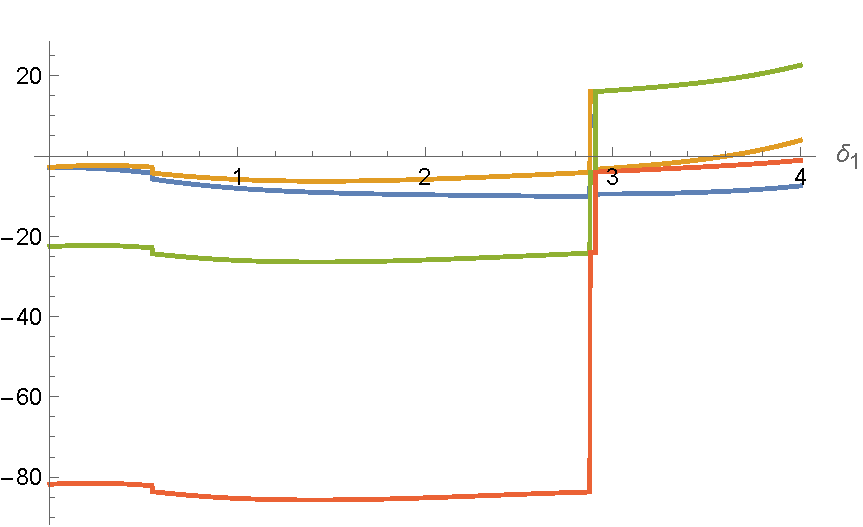
\includegraphics[scale=.55]{Chapters/discs.pdf}
  \end{subfigure}%
  \begin{subfigure}{.5\textwidth}
    \centering
    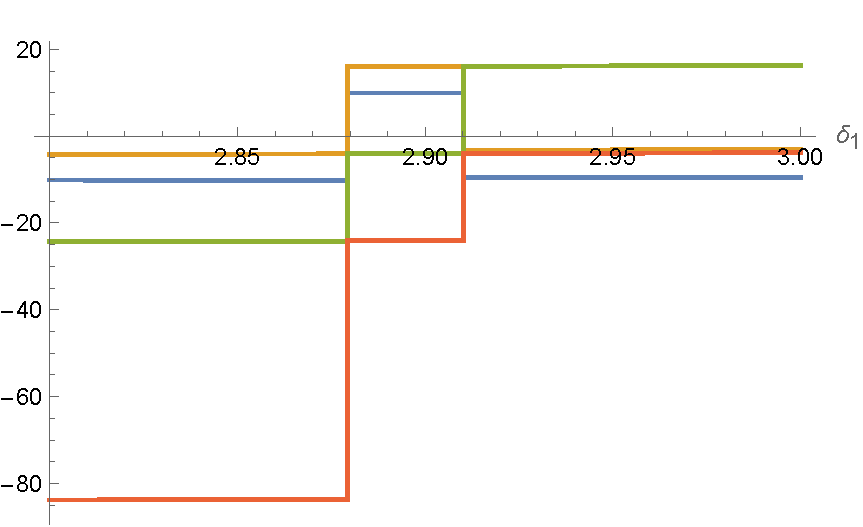
\includegraphics[scale=.55]{Chapters/discszoom.pdf}
  \end{subfigure}
  \caption{Discontinuities of lightcone block under analytic continuation~\eqref{eq:Reggelimitcoordinates}. In blue, the real part of the stripped-off lightcone block. In orange, the real part of the block with $\log(u_2)\to \log(u_2)+2\pi i$. In green, the previous with $\log(u_4)\to \log(u_4)-2\pi i$ and in red, the latter with $\log(u_5)\to \log(u_5)-2\pi i$. On the right, a zoomed-in version of the same plot. The plots are obtained with $\delta_2=0.73 \delta_1$. }
  \label{fig:discsforsimplecase}
\end{figure}
As we move according to the chosen path for analytic continuation, we observe that the lightcone block (blue) has discontinuities. The first one can be removed if one replaces $\log(u_2) \to \log(u_2)+ 2\pi i$ as shown by the orange line. Clearly, this shows that the discontinuity of the lightcone block is due to a logarithmic discontinuity in $u_2$. Similarly, when the orange line has a discontinuity, there is a continuation provided by the green line. The latter is defined from the former with the replacement $\log(u_4)\to \log(u_4)-2\pi i$. We conclude that a discontinuity in $u_4$ has taken place. The same is true for the red line which provides the continuation of the green line once we take $\log(u_5)\to \log(u_5)-2\pi i$ and once again a discontinuity, this time in $u_5$, has to be considered. This simple example shows in practice what we had already guessed: the lightcone block has discontinuities associated with $u_2, u_4$ and $u_5$ going around 0 and all of them are important. Let us then study the discontinuities of~\eqref{eq:simplecase} on these variables.

It is possible to use the integral representation of the lightcone block to argue that there are no sequential discontinuities involving $u_2$, i.e.
\begin{equation}
  \text{Disc}_{u_2} \text{Disc}_{u_4\, \text{or}\, u_5}G_{k_1,k_2, \ell} =\text{Disc}_{u_4\, \text{or}\, u_5}\text{Disc}_{u_2}  G_{k_1,k_2, \ell}=0\,.
\end{equation}
In the expression~\eqref{eq:simplecase} this is straightforward to see as there are no products of the type $\log(u_2)\log(u_4)$ or $\log(u_2)\log(u_5)$. As it was stated in the main text and as we will see below, it is actually the sum  $\text{Disc}_{u_2}  G_{k_1,k_2, \ell}+ \text{Disc}_{u_5}\text{Disc}_{u_4} G_{k_1,k_2,\ell}$ that dominates the Regge behaviour of the correlation function.

The discontinuity of expression~\eqref{eq:simplecase} as $u_2$ goes around 0 with fixed $u_4, u_5 >0$ is given by
\begin{equation}
  \pm 2\pi i\frac{u_1 u_3 u_5}{1-u_5+u_4(u_2 u_5-1)}\log\left(\frac{1-u_2}{(1-u_2 u_4)(1-u_2 u_5)}\right)\,,
\end{equation}
which in the limit $u_4, u_5 \to 1$ with $\chi_2=\frac{1-u_2}{(1-u_4)(1-u_5)}$ fixed simplifies to
\begin{equation}
  \label{eq:discu2simple}
  \pm 2 \pi i\frac{\sqrt{u_1} \sqrt{u_3}}{\left(\chi_2-1\right) \chi_4\chi_5}\log \left(\chi_2\right)\,,
\end{equation}
where we also use $\chi_4=\frac{1-u_4}{\sqrt{u_3}}$ and $\chi_5=\frac{1-u_5}{\sqrt{u_1}}$ which approach infinity due to the order of limits considered. This order of limits does not correspond to the actual Regge limit: indeed, we will call this ordered limit a boundary condition for Regge limit. The name simply follows from the fact that we use it below as a boundary condition for a set of recursion relations where we compute the Regge limit of a conformal block starting from the lightcone. Note, moreover, that the scaling in both $u_1$ and $u_3$ in the expression above agrees with the expected $u_i^{(1-J_i)/2}$ of Regge limit. As stated above we are indeed describing a double Reggeon exchange. This clearly contrasts with the Euclidean OPE scaling, $u_i^{\Delta_i/2}$, manifesting the difference between Regge and Euclidean kinematics. Perhaps a more striking example would follow from considering a spinning case from the beginning. The story is no different in those cases but the expressions grow considerably in size.
% Should we put this or not? \textbf{For a matter of compactness we avoid including them here but we provide an ancillary file with several examples of the explicit integrations including spinning contributions.}
We also note the existence of a $\log$ term in the case at hand. We point out that some other examples where the lightcone block can be integrated do not have these contributions in the above limit. Its existence in this case suggests however that a generic function for the discontinuity of the lightcone block as $u_2$ goes around 0 must contain $\log$ terms when the representation labels of the external and exchanged operators conspire in a certain way.

We now consider the discontinuity in $u_4$ with fixed and positive $u_2, u_5$. This gives
\begin{equation}
  \label{eq:discu4simplecomplete}
  \pm 2\pi i\frac{u_1 u_3 u_5}{1-u_5+u_4(u_2 u_5-1)}\log\left(\frac{1-u_4}{(1-u_2 u_4)u_5}\right)\,,
\end{equation}
which yields a boundary condition for Regge limit
\begin{equation}
  \label{eq:discu4simple}
  \pm 2 \pi i \frac{u_1 \sqrt{u_3}}{\chi_4}\,.
\end{equation}
From the symmetry of~\eqref{eq:simplecase} between $u_4$ and $u_5$ we immediately see that a similar result follows for the discontinuity in $u_5$. Note that these terms are subdominant in the limit $u_1, u_3 \to 0$ when compared to~\eqref{eq:discu2simple}. In particular, in expression~\eqref{eq:discu4simple} $u_1$ scales as $u_1^{\Delta_1/2}$ whereas $u_3$ scales as $u_3^{(1-J_2)/2}$. The converse happens in the discontinuity in $u_5$ complex plane. This behaviour should correspond to single Reggeon exchanges. Notably, the sequential discontinuity in $u_4$ and $u_5$ produces a dominant contribution for the double Reggeon kinematics. To see this, consider~\eqref{eq:discu4simplecomplete} and take the sequential discontinuity in $u_5$. This gives
\begin{equation}
  \pm 4 \pi ^2 \frac{u_1 u_3 u_5}{1-u_5+u_4 \left(u_2 u_5-1\right)}\,,
\end{equation}
which fixes the boundary condition for Regge limit
\begin{equation}
  4 \pi ^2\frac{\sqrt{u_1} \sqrt{u_3}}{\left(\chi _2-1\right) \chi _4 \chi _5}\,,
\end{equation}
that is as dominant as~\eqref{eq:discu2simple}. We conclude in this simple example, the generic statement we have made in the main text that $\text{Disc}_{u_2}  G_{k_1,k_2, \ell}+ \text{Disc}_{u_5}\text{Disc}_{u_4} G_{k_1,k_2,\ell}$ provide the dominant contributions of the correlation function in Regge limit.

Even though the existence of $\log$ terms in the boundary condition for the Regge limit is not generic, we should however show how to deal with them when we compute the conformal blocks at Regge limit. If there are no $\log$ terms in your case of interest, simply set those terms to zero in the procedure below.
We consider the Casimir equations in the limit of $u_1, u_3 \to 0$ with a block that scales as
\begin{equation}
  \mathcal{G}_{k_{1}^{\prime} k_{2}^{\prime}\ell}(x_i) \propto u_1^{\frac{1-J_1}{2}} u_3^{\frac{1-J_2}{2}}\mathcal{H}(\chi_2,\chi_4,\chi_5)\,\,.
\end{equation}
In this limit, the Casimir equations for $\mathcal{H}$ simplify and read
\begin{align}
  \label{eq:casinHregge}
   & \left[\chi_4^2 \left(4 (2\chi_2-1) (\partial_{\chi_2}-\chi_5 \partial_{\chi_2}\partial_{\chi_5})-(d-1) \chi_5^3 \partial_{\chi_5}-\left(\chi_5^2-4\right) \chi_5^2 \partial_{\chi_5}^2\right)\right.\nonumber \\
   & \left.+4\left((\chi_2-1) \chi_2 \chi_4^2+1\right)\partial_{\chi_2}^2+(\Delta_1-1)(\Delta_1-d+1)\chi_4^2 \chi_5^2\right]\mathcal{H}(\chi_2,\chi_4,\chi_5)=0
\end{align}
with an entirely similar second equation obtained from the above by replacing $\Delta_1$ by $\Delta_2$ and permuting the roles of $\chi_4$ and $\chi_5$. In our particular case of study, in the limit of $u_1, u_3 \to 0$, large $\chi_4, \chi_5$ and fixed $\chi_2$, the leading Regge contribution of the block behaves as
\begin{equation}
  \label{eq:bdycondition222}
  \frac{\sqrt{u_1}\sqrt{u_3}}{(\chi_2-1)\chi_4 \chi_5}\left(a+b \log(\chi_2)\right)
\end{equation}
where $a$ and $b$ are constants. We can thus further impose in~\eqref{eq:casinHregge}
\begin{equation}
  \mathcal{H}(\chi_2,\chi_4,\chi_5)=\frac{\mathbb{H}(\chi_2,\chi_4,\chi_5)}{\chi_4  \chi_5}\,.
\end{equation}
According to~\eqref{eq:bdycondition222} and considering a small-$\chi_2$  limit, we can look for solutions of the Casimir equations of the form
\begin{equation}
  \mathbb{H}(\chi_2,\chi_4,\chi_5)=\sum_{n_1,n_2,n_3} a_{n_1,n_2,n_3} \chi_2^{n_1} \chi_4^{-n_2} \chi_5^{-n_3}+ b_{n_1,n_2,n_3} \log(\chi_2) \chi_2^{n_1} \chi_4^{-n_2} \chi_5^{-n_3}
\end{equation}
where the coefficients $a_{n_1,n_2,n_3}$ and $b_{n_1, n_2,n_3}$ reduce to $a$ and $b$, respectively, when all $n_i$ are 0. The remaining expansion coefficients $a_{n_1,n_2,n_3}$ and $b_{n_1, n_2,n_3}$ are fixed by the Casimir equations. It is easy to see that this ansatz gives rise to terms in the Casimir equations of the form
\begin{equation}
  \chi_2^{c_1+n_1}\chi_4^{c_2-n_2} \chi_5^{c_3-n_3}\times\begin{cases}a_{n_1,n_2,n_3} \\
    b_{n_1,n_2,n_3} \\
    b_{n_1,n_2,n_3}\log(\chi_2)\end{cases}\,.
\end{equation}
Clearly, the terms that depend on $\log$ should cancel among each other in order to satisfy the Casimir equation. This leads to two constraints per Casimir equation, one for the $\log$-dependent terms and one for the remaining. For the isolated $\log$ terms, we find recursion relations for the coefficients by removing the $\chi$-dependence from the equations. To do so, we shift each term accordingly, i.e. $n_1 \to n_1-c_1, n_2 \to n_2+c_2$ and $n_3 \to n_3+ c_3$. This leads to the following recursion relations
\begin{align}
  b_{n_1,n_2,n_3}= \frac{1}{n_3 (d-n_3-4)} & \left[ 4 (n_1+1) \left((n_1+n_3)
    b_{n_1+1,n_2,n_3-2}-(n_1+2)
  b_{n_1+2,n_2-2,n_3-2}\right)\right.\nonumber                                \\
                                           & \left. -4 (n_1+n_3-1) (n_1+n_3)
    b_{n_1,n_2,n_3-2}\right]
\end{align}
with a similar one where we exchange the roles of $n_3$ and $n_2$. Clearly, the above recursion relation cannot be used whenever $n_3=0$. In such case, the other recursion relation can be used instead (and vice-versa). An entirely similar argument follows for the non-$\log$-dependent terms. We find the recursion relations
\begin{align}
   & a_{n_1,n_2,n_3}= \frac{4}{n_2 (4-d+n_2)}\left[(n_1+n_2-1) (n_1+n_2)
    a_{n_1,n_2-2,n_3}-(n_1+1) (n_1+n_2)
  a_{n_1+1,n_2-2,n_3}\right.\nonumber                                    \\
   & \left.+(n_1+1) (n_1+2)
    a_{n_1+2,n_2-2,n_3-2}+(2 n_1+2 n_2-1)
    b_{n_1,n_2-2,n_3}-(2 n_1+n_2+1)
  b_{n_1+1,n_2-2,n_3}\right.\nonumber                                    \\
   & \left.+(2 n_1+3)
    b_{n_1+2,n_2-2,n_3-2}\right]
\end{align}
with another equivalent relation where the roles of $n_2$ and $n_3$ are swapped.

These recursion relations are only meaningful once one prescribes a boundary condition. We impose that
\begin{align}
   & a_{n_1,n_2,n_3}=b_{n_1,n_2,n_3}=0\qquad \text{if} \qquad n_1<0\, \lor\, n_2<0\, \lor\, n_3<0\,,\nonumber \\
   & a_{0,0,0}= a \qquad \text{and} \qquad b_{0,0,0}=b\,.
\end{align}
It is easy to check that these recursion relations fix the behaviour of all the coefficients up to those of the form $a_{n_1,0,0}$ and $b_{n_1,0,0}$ but note that these can be read from~\eqref{eq:bdycondition222} by expanding it on small $\chi_2$ limit.

\section{Other Regge kinematics}
\label{sec:otherregge}
In this short appendix, we detail other possible Regge kinematics that we did not explore in detail in this paper but that might be worth studying in the future.

\subsubsection*{Single Reggeon exchange}

Within a five-point function, one can consider a single Reggeon exchange. In terms of Mandelstam invariants $s_{25}$ or $s_{45}$ of figure~\ref{fig:mandelstaminv5pt} only one of the two becomes large. In the context of CFTs, this translates to having only two operators, one in the first and one in the second Poincare patches, approaching each other in such a way that there is only one cross-ratio going to $0$ rather than two.

One possible analytic continuation that describes single Reggeon exchange is given by
\begin{align}
   & x_{1}= -r\left(\sinh(\delta_1), \cosh(\delta_1), \textbf{0}_{d-2} \right)\, &  & x_{3}= \left(0, 1, \textbf{0}_{d-2} \right)\,   & x_5=(0,h_1,h_2,\textbf{0}_{d-3})\nonumber \\
   & x_{2}= r\left(\sinh(\delta_2),  \cosh(\delta_2), \textbf{0}_{d-2} \right)\, &  & x_{4}= \left(0, -1, \textbf{0}_{d-2} \right)\,.
\end{align}
with positive rapidities $\delta_i$ and $\textbf{0}_{d}$ denoting a $d$-dimensional vector of zeros. In the large-rapidities limit, one can check that $u_1 \to 0$ and $u_2, u_5 \to 1$ with unfixed $u_3$ and $u_4$. This agrees with the Euclidean OPE limit in the (12) channel. Again, we emphasize that this limit is attained after branch-cuts are crossed and thus in an intrinsically Lorentzian Regge sheet.

\subsubsection*{Six-point snowflake}

The six-point conformal block of external scalars is known in the lightcone limit in the snowflake topology~\cite{Antunes:2021kmm}. Even though we did not attempt in this paper to analyse the cut-structure of this block, we nonetheless write down an analytic continuation prescription to achieve a Regge limit configuration that is consistent at the level of the cross-ratios with the OPE on channels (12), (34) and (56).

We use the set of 9 cyclic cross-ratios
\begin{align}
   & u_1=\frac{x_{12}^2 x_{35}^2}{x_{13}^2 x_{25}^2} \quad u_{i+1}=u_i\vert_{x_i\to x_{i+1}} \quad \text{mod 6}\,\nonumber \\
   & U_1=\frac{x_{13}^2 x_{46}^2}{x_{14}^2 x_{36}^2}\quad U_{i+1}=U_i\vert_{x_i\to x_{i+1}} \quad \text{mod 3}\,.
\end{align}
In the snowflake OPE limit $u_1, u_3, u_5 \to 0$ and the remaining all go to 1. In the Regge limit one should reobtain the same limiting values of the cross-ratios after some lightcones are crossed. We start with a totally spacelike configuration and perform the analytic continuation
\begin{align}
  \label{eq:analyticcont6pt}
   & x_{1}= -r_1\left(\sinh(\delta_1),\cosh(\delta_1), \textbf{0}_{d-2} \right)\, &  & x_{4}= \left(\sinh(\delta_1), -\cosh(\delta_1), \textbf{0}_{d-2}\right)\,\nonumber \\
   & x_{2}= r_1\left(\sinh(\delta_2),\cosh(\delta_2), \textbf{0}_{d-2}\right)\,   &  & x_5=(r_2\sinh(\delta_3), r_3, h, r_2 \cosh(\delta_3),\textbf{0}_{d-4})\nonumber\,  \\
   & x_{3}= \left(-\sinh(\delta_2), \cosh(\delta_2), \textbf{0}_{d-2} \right)\,   &  & x_6=(-r_2 \sinh(\delta_3), r_4, h,- r_2 \cosh(\delta_3),\textbf{0}_{d-4})\,.
\end{align}
where one can see that we use 9 degrees of freedom. Note as well that for six-point functions one can at most use the conformal symmetry to state that any generic correlation function is related to one that lives in some half-subspace in 4 dimensions~\cite{Kravchuk:2016qvl}. Perhaps the most notorious difference in this case is the need to boost a pair of points along some different plane. It is easy to check however that this prescription indeed leads to the expected OPE behaviour for a snowflake six-point function.

% % \bibliographystyle{unsrt}
% \nocite{*}
% % \printbibliography


\cleardoublepage
